\newgeometry{top=1 in, bottom=1 in, left=1.5 in, right=1.5 in}

\subsection{Simulering}
Resultaterne fra analysen simuleres med diagrammerne vist i Figur  og Figur . 

\subsubsection{Simulering af 1. ordens lavpasfilter}
Figur viser simuleringen af 1. ordens lavpasfilter. På oscilloskopet vises kurveformen for $V_out$ og heraf bestemmes tidskonstan for R = 10 k$Omega$ og R = 100k$Omega$.
I de to tilfælde bestemmes den maksimale værdi af $V_out$
Resultaterne indføres i tabel 1.

\begin{figure}[h]
 \begin{center}
  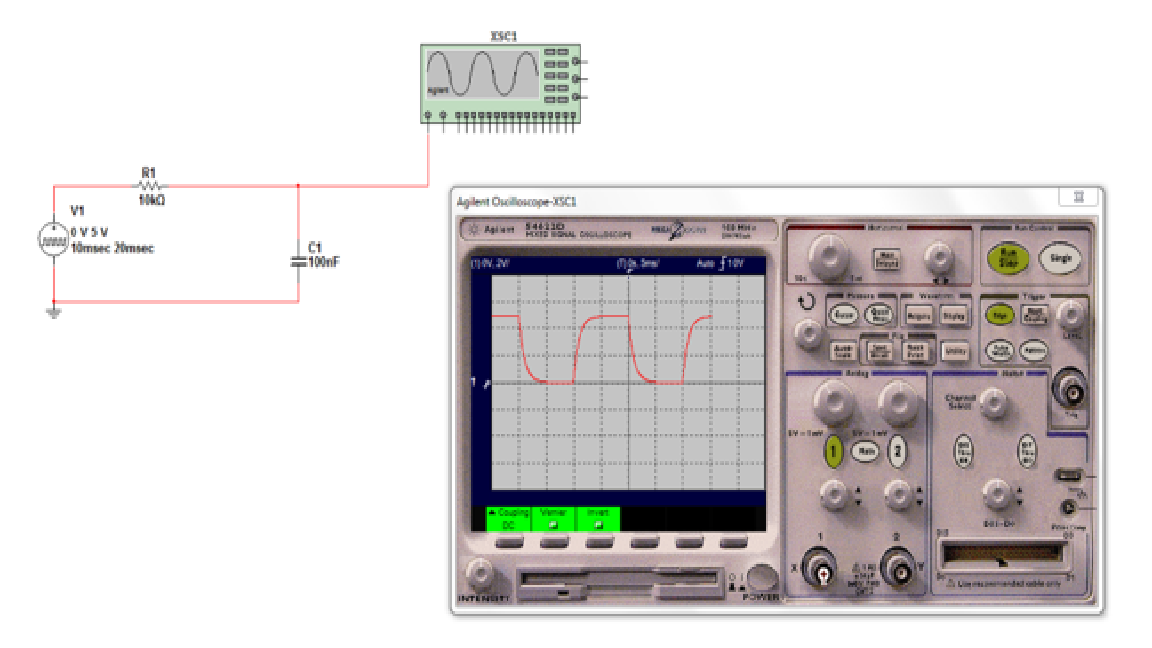
\includegraphics[height=5cm]{P_Figur/1.orden}
  \caption{}
  \label{fig:}
 \end{center}
\end{figure}